\documentclass{article}
\usepackage[utf8]{inputenc}
\usepackage{graphicx}
\usepackage{blindtext}
\usepackage{subfiles}
\usepackage[colorlinks = false]{hyperref}
\usepackage[table]{xcolor}
\usepackage{rotating}
\usepackage{adjustbox}


\usepackage[TS1,T1]{fontenc}

\usepackage[
backend=biber,
style=authoryear,
citestyle=authoryear
]{biblatex}
\renewcommand*{\bibfont}{\footnotesize}
\usepackage[normalem]{ulem}
\usepackage{fancyhdr}
\pagestyle{fancy}
\fancyhf{}
\rhead{Measuring Rhetorical Similarity - Appendix}
\lhead{Nicolai Berk}
\cfoot{\thepage}

\useunder{\uline}{\ul}{}

\addbibresource{refs.bib}


\title{ONLINE AppENDIX\newline Measuring Rhetorical Similarity with Supervised Machine Learning}
\author{Nicolai Berk}
\date{\today}


\begin{document}


\subsection*{Appendix A}

\begin{table}[ht!]
\noindent\adjustbox{max width=\textwidth}{%
\begin{tabular}{|l|l|l|l|l|l|l|}
\hline
\textbf{Classifier}   & \textbf{Vectorizer} & \textbf{Stemmed} & \textbf{F1}   & \textbf{Accuracy} & \textbf{Precision} & \textbf{Recall} \\ \hline
Logistic   Regression & tfidf               & raw              & \textbf{0.59} & 0.87              & 0.55               & 0.64            \\ \hline
SVM                   & tfidf               & raw              & \textbf{0.57} & 0.88              & 0.59               & 0.56            \\ \hline
Logistic   Regression & tfidf               & stemmed          & \textbf{0.55} & 0.83              & 0.45               & 0.7             \\ \hline
Multinomial NB        & tfidf               & raw              & \textbf{0.55} & 0.85              & 0.48               & 0.64            \\ \hline
Multinomial NB        & tfidf               & stemmed          & \textbf{0.54} & 0.84              & 0.47               & 0.64            \\ \hline
SVM                   & tfidf               & stemmed          & \textbf{0.54} & 0.84              & 0.47               & 0.62            \\ \hline
Logistic   Regression & count               & raw              & \textbf{0.49} & 0.84              & 0.46               & 0.53            \\ \hline
Logistic   Regression & count               & stemmed          & \textbf{0.48} & 0.83              & 0.43               & 0.55            \\ \hline
Multinomial NB        & count               & raw              & \textbf{0.46} & 0.85              & 0.48               & 0.45            \\ \hline
Multinomial NB        & count               & stemmed          & \textbf{0.46} & 0.85              & 0.47               & 0.45            \\ \hline
SVM                   & count               & raw              & \textbf{0.46} & 0.83              & 0.42               & 0.5             \\ \hline
SVM                   & count               & stemmed          & \textbf{0.45} & 0.81              & 0.4                & 0.52            \\ \hline
\end{tabular}
}
\caption{Performance of different qualifiers on German data, sorted by F1-score. $F_1 = 2*\frac{precision*recall}{precision+recall}$ }
\end{table}

\newpage


\subsection*{Appendix B}

The Netherlands saw only one formal coalition government between radical-right and centre-right, but an additional minority government supported by the radical-right PVV. In 2002 the \textit{Lijst Pim Fortuyn} (LPF) brought unprecedented volatility and polarisation into Dutch politics (\cite{Bischof2019a, VanderBrug2003}). Only formed about three months preceding the election, the party gained wide attraction due to its charismatic leader, its distinctive anti-immigration stance, and voters' alienation with established parties on the centre-right and -left (\cite{Lucardie2007LPF, Pennings2003}). On election day, nine days after the party leader Pim Fortuyn was assassinated, the party came in second with 17\% of the vote and formed a coalition with the christian-democrat CDA and the centre-right VVD. Having lost its founding father and as a result of its rapid success, the party was unprepared for government and turmoiled by internal power struggles. This peaked when two LPF ministers stopped talking to each other. As a result, CDA and VVD broke the coalition only 87 days after its formation (\cite{DeLange2011, Heinisch2003, Lucardie2007LPF}). I expect especially the LPF to become more similar to VVD and CDA here, as the party members decide to enter a coalition government. Similarly, VVD and CDA should become more alike the LPF in government.\par

The co-operation of VVD, CDA and PVV in 2010 did not result in a formal majority coalition (partly due to internal conflicts in the CDA regarding a coalition with the radical-right PVV), but a 'supported minority government'. This was the first minority government formed in the Netherlands since 1922. VVD and CDA staffed the cabinet, while the PVV only promised support on major issues. As this support was settled in a formal agreement, this government became basically a 'majority government in disguise' (\cite{Strom1990, VanHolsteyn2011}). In fact, the government cooperated very little with the opposition even compared to full majority governments - this is likely an outcome of the sorting of parties into a right-wing government and a left-wing opposition but underlines the similarity of this government to classic majority coalitions (\cite{Otjes2014}). As a result, I expect an increased similarity of the coalition partners, slightly less than in a majority coalition. \par

\begin{figure}[ht!]
    \begin{minipage}{\textwidth}
    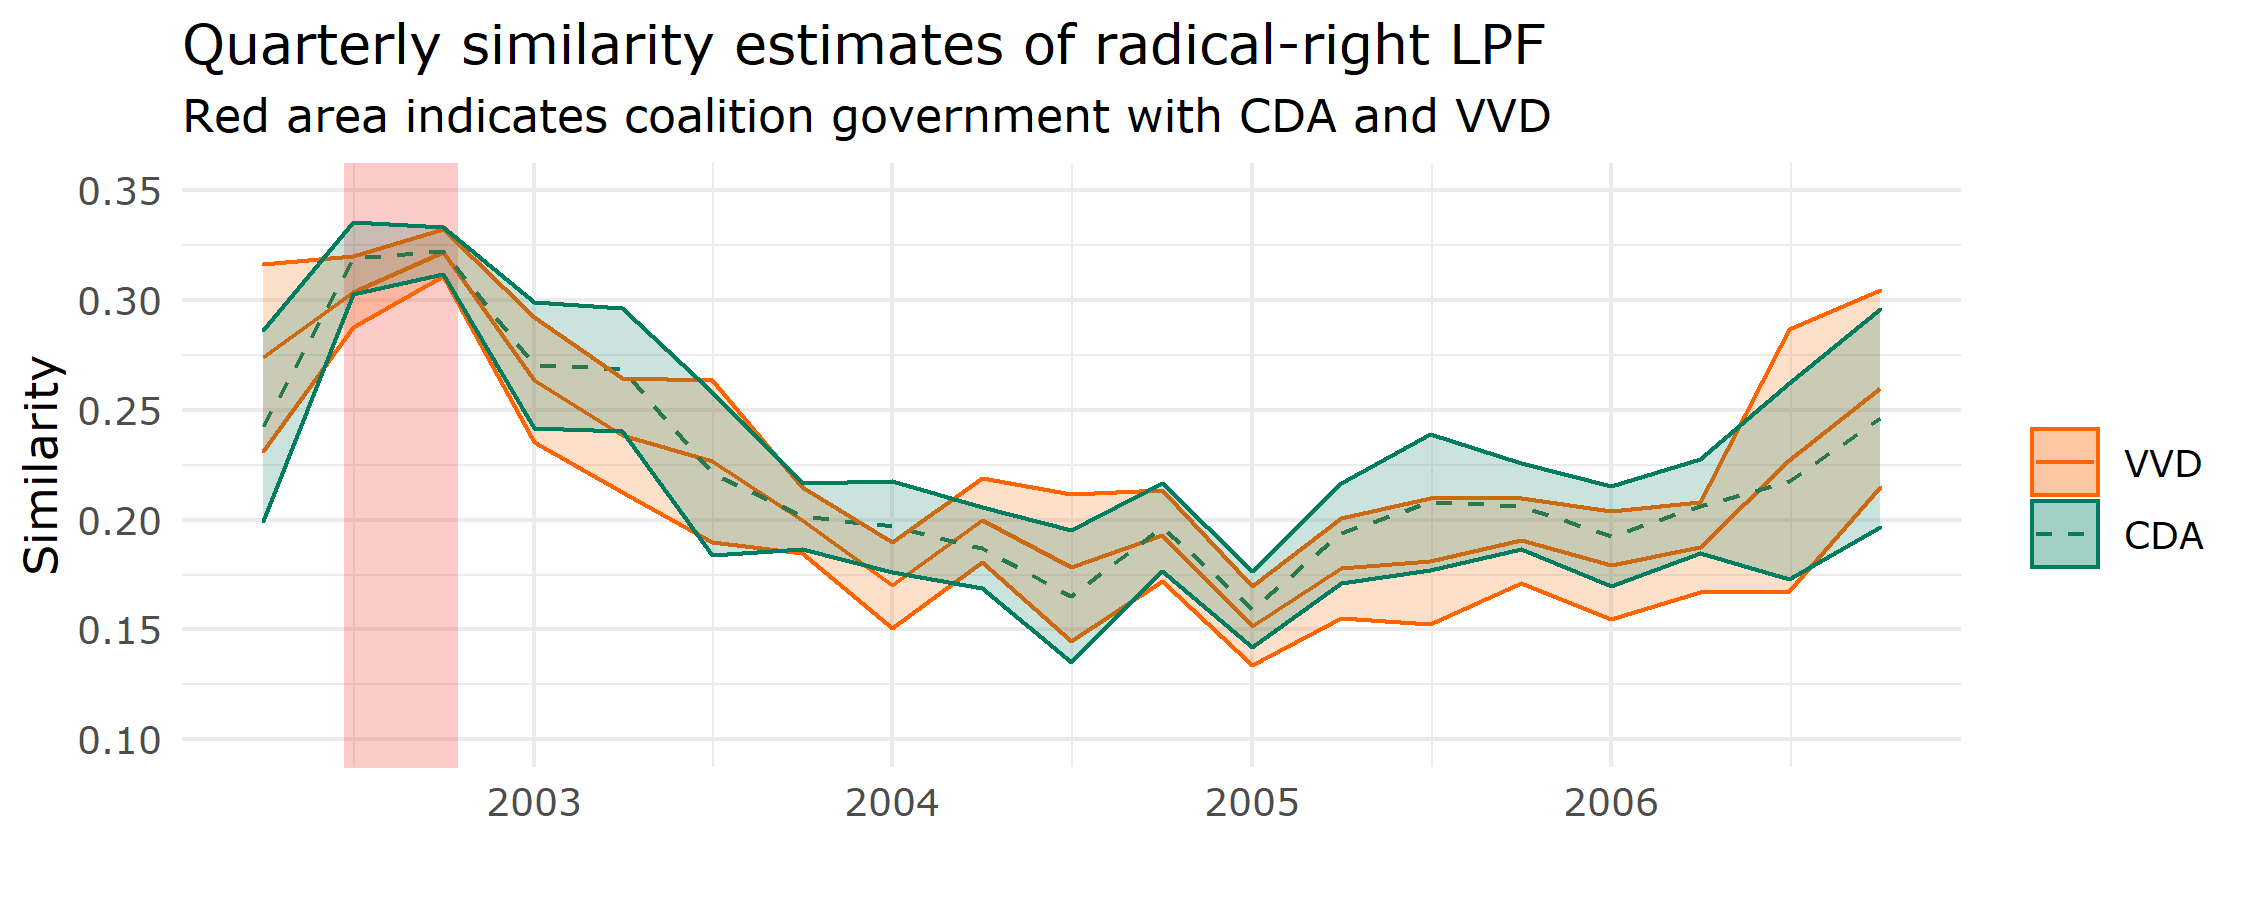
\includegraphics[width=\linewidth]{NL/vis/NL_lpf_sim.png}
    \end{minipage}
    \hfill
    \begin{minipage}{\textwidth}
    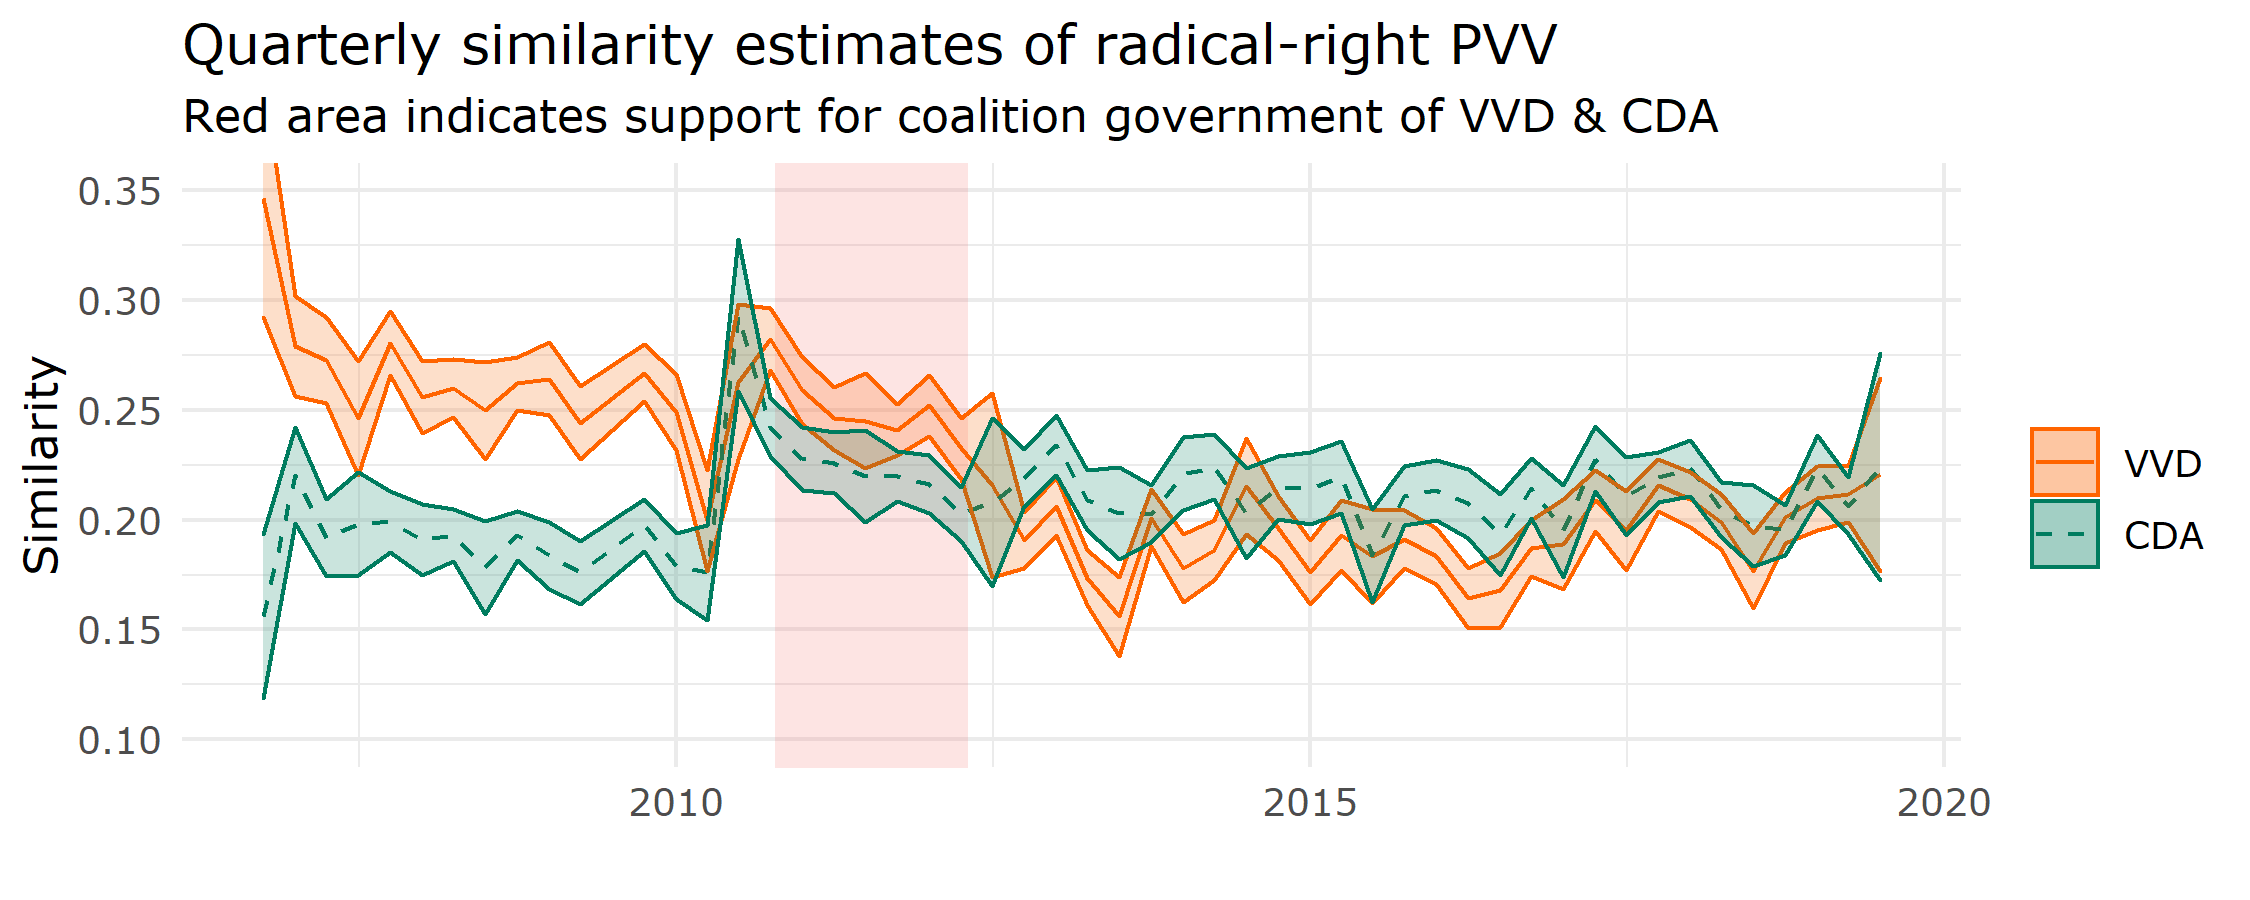
\includegraphics[width=\linewidth]{NL/vis/NL_pvv_sim.png}
    \end{minipage}
    \caption{Similarity of radical-right LPF (top) and PVV (bottom) towards their coalition partners across time.}
    \label{fig:nl_RR}
\end{figure}

The top row of figure \ref{fig:nl_RR} shows the average similarity of the LPF towards CDA and VVD per quarter. The red-shaded area indicates the period in which the three parties governed together. A first glimpse reveals how closely the two estimates track each other. The LPF is rather similar to the two coalition partners when in government, obtaining a similarity estimate of about 30\% throughout the time governing. Once the party leaves the government, the similarity decreases again, before becoming slightly more similar again briefly before its dissolution. For the PVV (bottom row figure \ref{fig:nl_RR}), a more complicated picture emerges. As the PVV was formed by a former member of the VVD, it is not surprising that the similarity towards the liberal party - compared to the CDA - is somewhat higher after the PVV's formation. This changes preceding the government formation in 2010. At first, the similarity to the VVD steeply declines to the CDA's level (about 20\%), before the similarity to both centre-right parties increases steeply to about 35\% just before the government formation. This might reflect higher distinctiveness during electoral campaigns, before an accommodation surrounding coalition talks. During the phase in government, the similarity slowly decreases to pre-formation levels. Interestingly, the similarity towards VVD and CDA lie at similar levels (around 20\%) now, the similarity towards the CDA even seems slightly higher. \par

\begin{figure}[ht!]
    \hfill
    \begin{minipage}{\textwidth}
    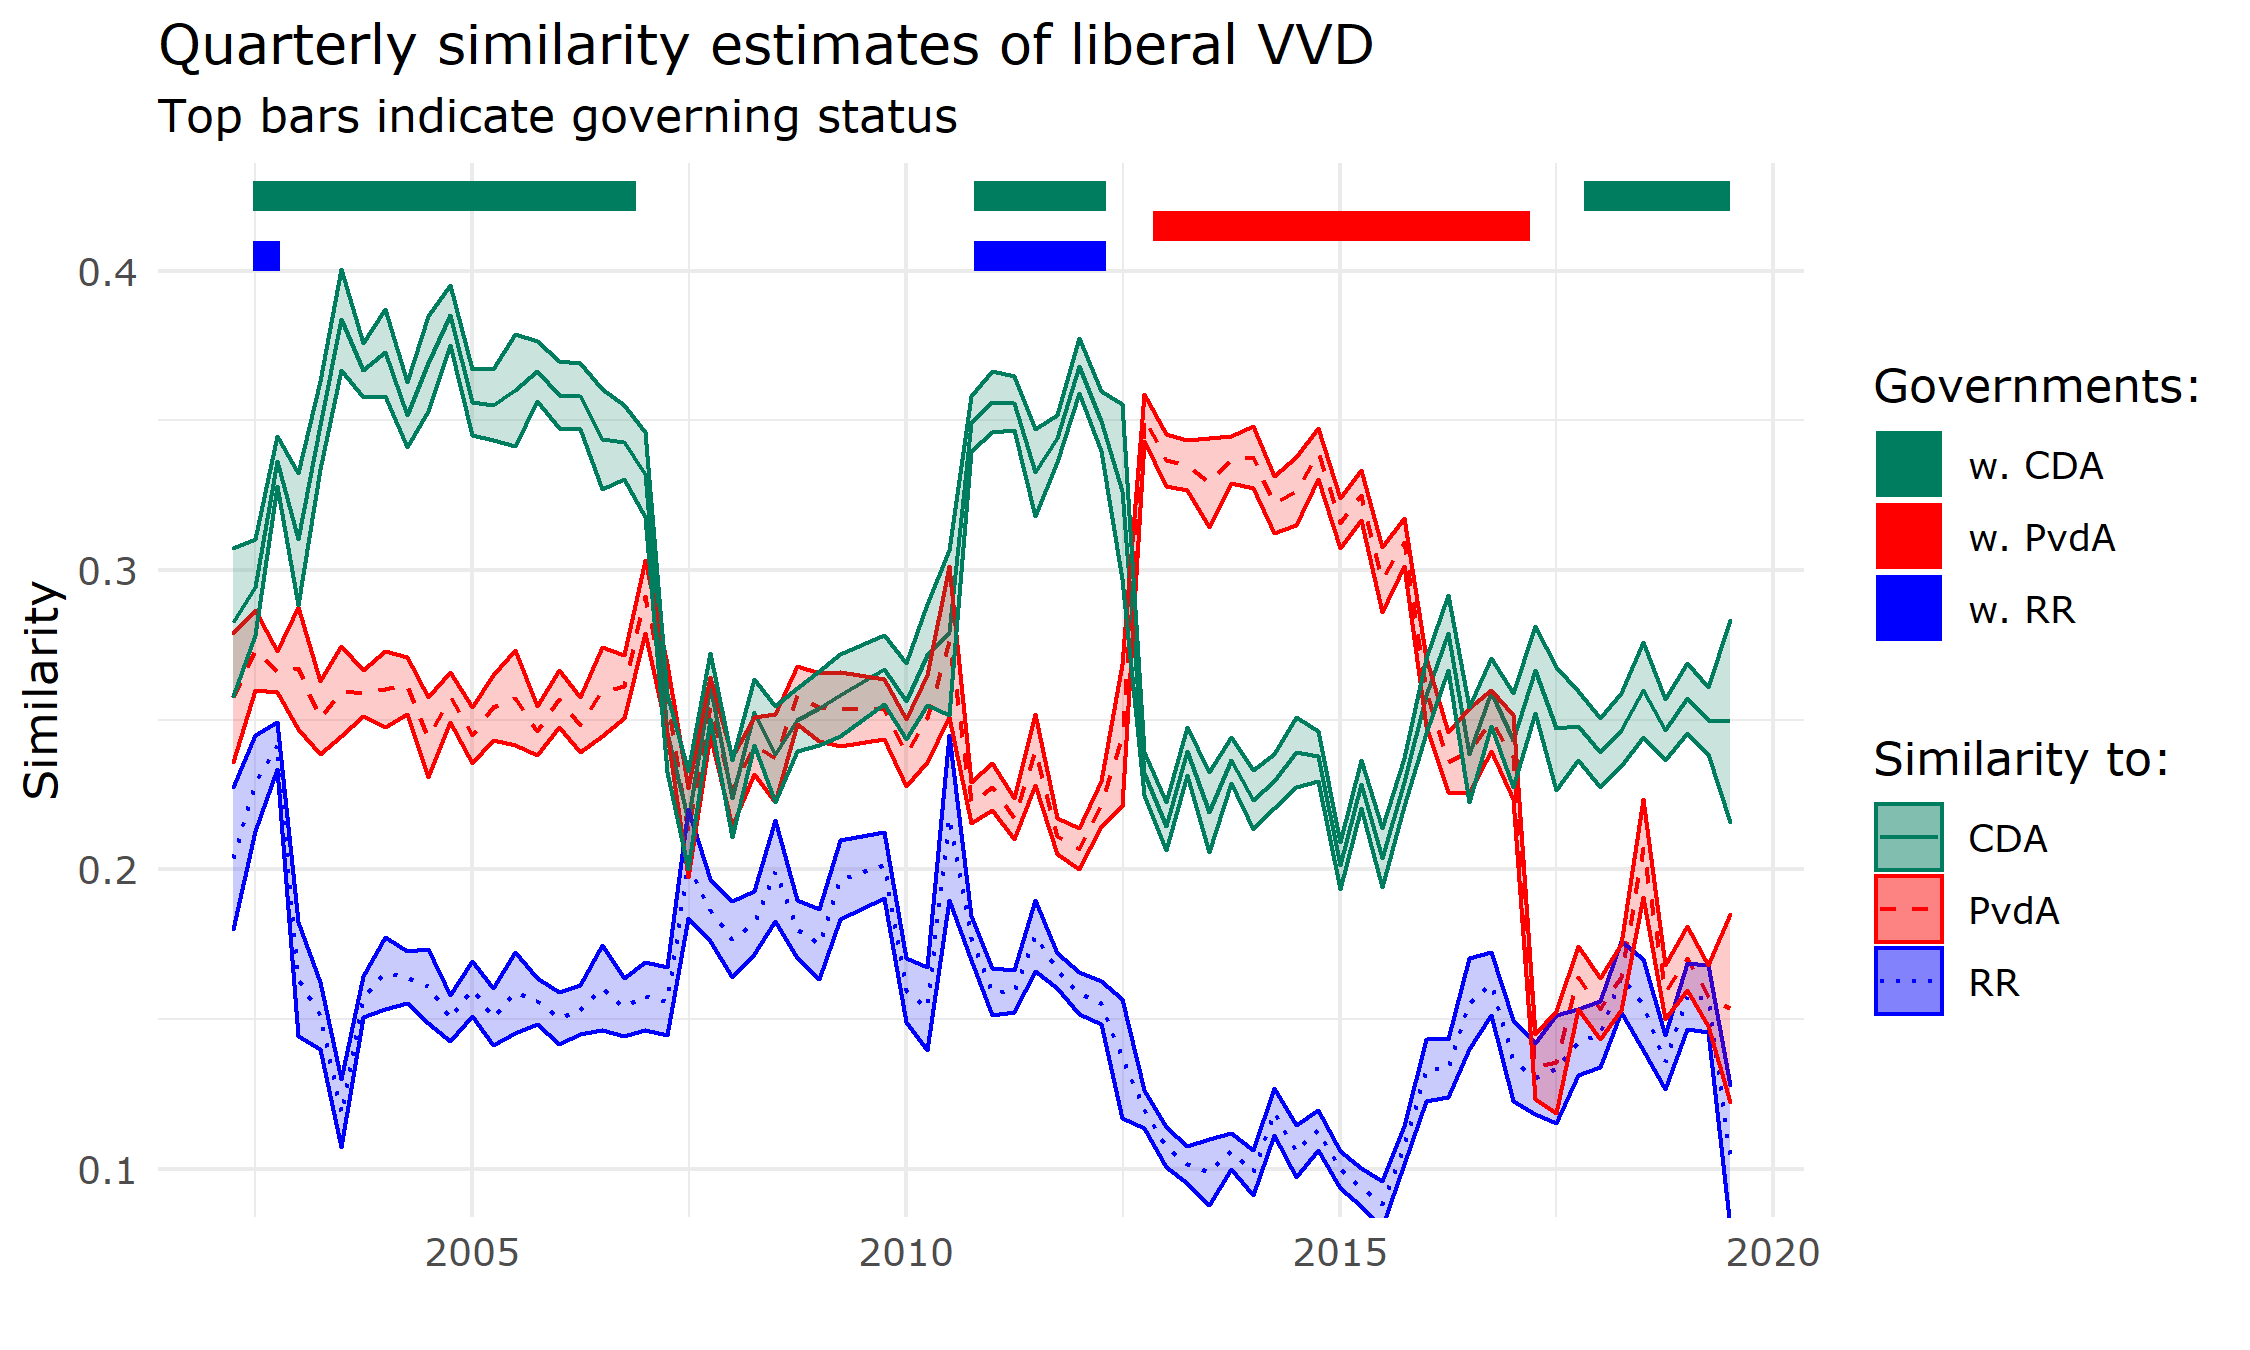
\includegraphics[width=\linewidth]{NL/vis/NL_vvd_sim.png}
    \end{minipage}
    \hfill
    \begin{minipage}{\textwidth}
    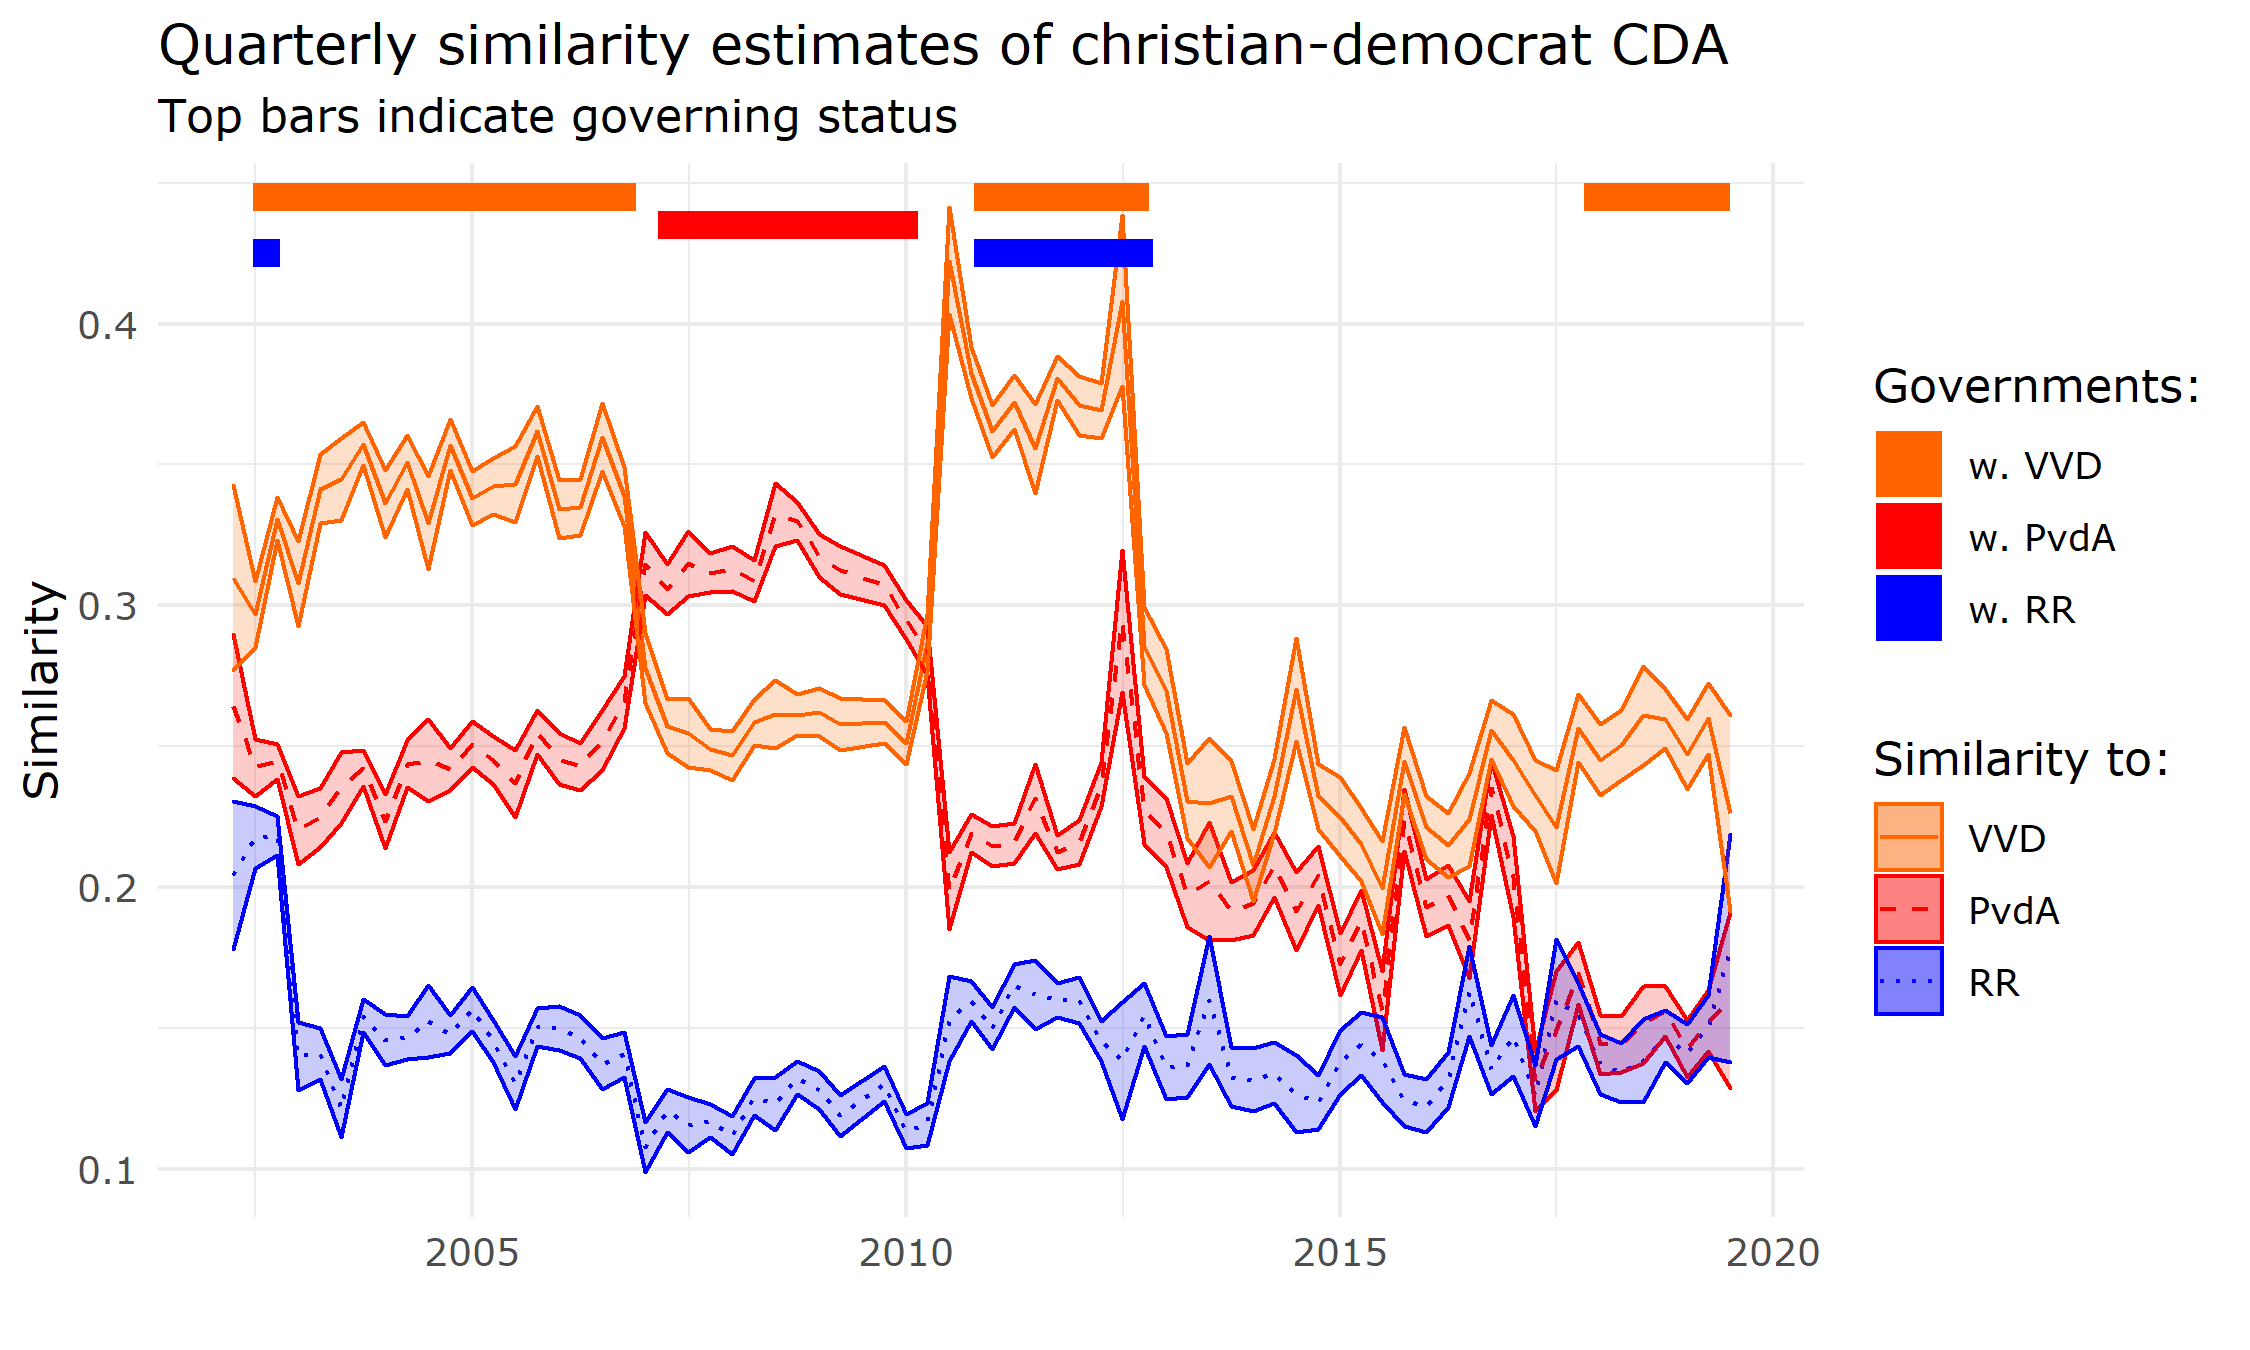
\includegraphics[width=\linewidth]{NL/vis/NL_cda_sim.png}
    \end{minipage}
    \caption{Similarity estimates for VVD and the two major radical-right parties.}
    \label{fig:nl_CR}
\end{figure}

Figure 2 displays the estimates for the liberal VVD (top) and chrstian-democrat CDA (bottom). The bars in the top indicate which parties were governing in coalition with the party at the time, as indicated by the order and colors in the legend on the top-right. So for the VVD (top graph), top (green) bars from 2002-2007, 2010-2012, and 2017-2019 indicate that the party was governing in coalition with the CDA at the time. The second row (red bar) indicates when the party was governing with the social-democrat PvdA, and the blue bars in the bottom row indicate support from radical-right parties. The graph below indicates the similarity towards the parties indicated in the legend on the bottom-right. A first observation indicates substantial variation in the similarity estimates. Until recently, the two centre-right parties show higher similarity to centrist parties compared to the radical-right. Comparing the bars in the top to the graphs, it becomes evident that higher estimates correspond to governing periods of the respective parties. The VVD displays higher similarity to the CDA (and vice versa) when in coalition government with the party, with the exception of the most recent coalition. Here the shift takes place earlier and does not reach similarity comparable to other coalitions. This might indicate the lesser room for accommodation in a four-party coalition. The similarity of the two centre-right parties towards the PvdA shows similar patterns (higher estimates in coalitions), however an additional observation can be made: preceding the governments with PvdA participation in 2007 and 2012, both the VVD and CDA show increased similarity preceding the formations, irrespective of whether the party actually became part of the coalition. For the radical-right, the pattern indicates clearly heightened similarity towards the LPF during its brief government participation, while the coalition with the PVV is only visible in the CDA estimates - the VVD accommodates the radical-right party prior to the formation, but returns to prior similarity during the coalition. Additionally, governing with the social democrats seems to decrease the similarity to the radical-right. \par

T-tests confirm these observations. The monthly average similarity of the LPF towards VVD and CDA increases substantially while in government (VVD: $+9pp$\footnote{Percentage points}; CDA: $+10.6pp$), however only reaches conventional levels of significance for the CDA ($p < 0.001$). The PVV shows lower accommodation to the established parties, similarly differing in significance (VVD: $+3.1pp; p < 0.001$; CDA: $+1.4pp; p > 0.01$). CDA and VVD accommodate towards the radical-right when governing with these parties (VVD: $2.7pp; p < 0.001$; CDA: $3pp; p < 0.001$), however the effect is much stronger when in coalition with the LPF (VVD: $8.3pp; p < 0.001$; CDA: $7.5pp; p < 0.001$) than when supported by the PVV (VVD: $1.5pp; p< 0.001$; CDA: $2.1pp; p< 0.001$). Similarity towards each other is similarly affected when governing with each other (VVD: $+7.4pp$; CDA $5.8pp$; both $p < 0.001$), as well as the similarity towards the PvdA when governing with this party (VVD: $+3.3pp$, CDA: $+8.8pp$). Interestingly, governing with the social democrats also affects the similarity towards the radical-right negatively (VVD: $-4.7pp$; CDA: $-2.4pp$; both $p<0.001$). This is especially striking as the effect for the VVD is \textit{twice} the size compared to governing with a radical-right party. \par

The main expectation is confirmed by these findings: coalition parties accommodate towards each other, validating the measurement. However, additional interesting variation can be observed: a lot of variation is produced in the context of government formations, where parties accomodate likely coalition partners. Similarly, while the centre-right showed higher similarity to the social-democrats compared to the radical right, this no longer seems to be the case. This is especially relevant as the PvdA seemed to function as a safeguard against radical-right accommodation when governing with the centre-right, substantially decreasing the centre-rights similarity to the radical-right.

\newpage

\subsection*{Appendix C}
\begin{table}[ht!]
\begin{tabular}{|l|l|l|l|}
\hline
Word        & Contribution & Word           & Contribution \\ \hline
minister    & 50.2         & mij            & 8.4          \\ \hline
kunnen      & 16.5         & kabinet        & 8.2          \\ \hline
vind        & 15.8         & hij            & 7.8          \\ \hline
Algerije    & 12           & ministerie     & 7.3          \\ \hline
ben         & 11.7         & Het            & 7.1          \\ \hline
motie       & 10.8         & Arabië         & 7.1          \\ \hline
LPF         & 10.7         & imam           & 7            \\ \hline
AIVD        & 9.9          & terroristische & 6.9          \\ \hline
Wij         & 9.9          & groot          & 6.9          \\ \hline
zeker       & 9.6          & Europa         & 6.8          \\ \hline
mening      & 9.6          & onderzoek      & 6.2          \\ \hline
Defensie    & 9.5          & Dutchbat       & 6.2          \\ \hline
terroristen & 9.4          & man            & 6            \\ \hline
Dat         & 9.3          & moskeeën       & 5.6          \\ \hline
Saoedi      & 8.6          & moskee         & 5.5          \\ \hline
\end{tabular}
\caption{Thirty words with the strongest positive contribution in Wilders' speeches as a member of the VVD 2004.}
\label{tab:wilders}
\end{table}

\newpage

\printbibliography



\end{document}